\begin{figure}[h]
\uwsinglespace
\centering
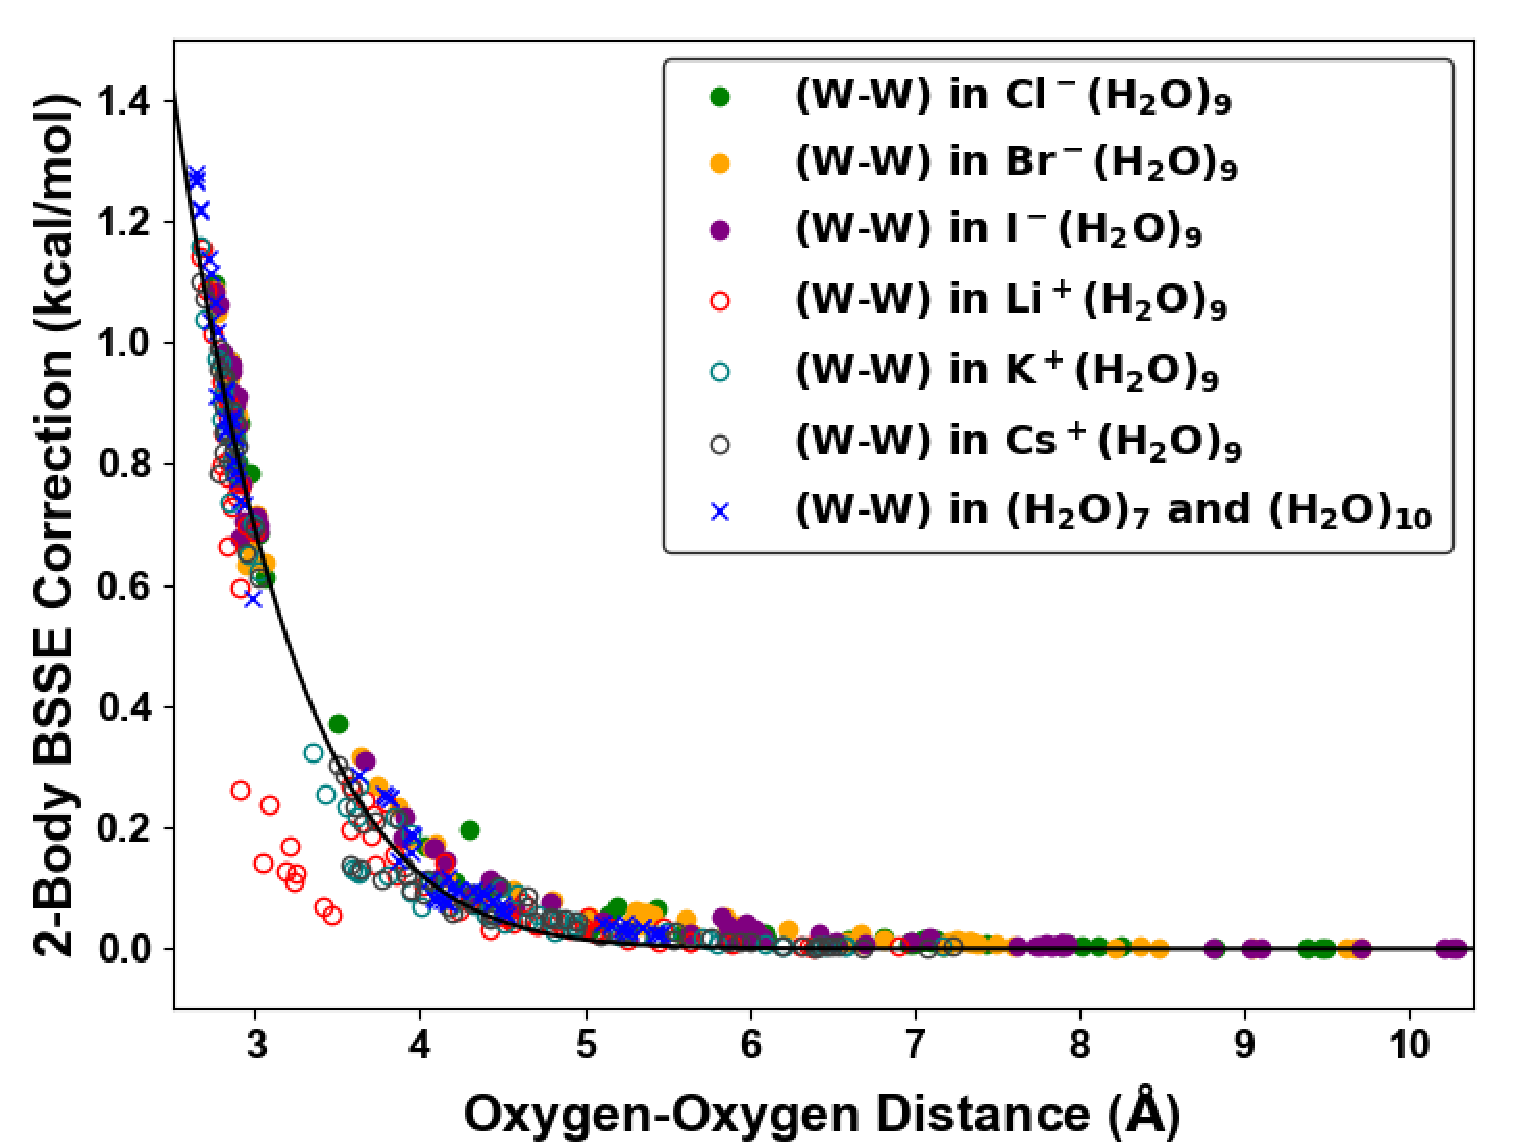
\includegraphics[width=.8\textwidth]{Figures/Chapter_3/figure_10.pdf}
\caption[2-Body BSSE correction for all 498 water dimers extracted from the \ce{Z^{+/-}(H2O)9}, \ce{Z} = \ce{Li^+}, \ce{K^+}, \ce{Cs^+}, \ce{Cl^-}, \ce{Br^-}, \ce{I^-}, clusters as well as the two neutral water clusters \ce{(H2O)7} and \ce{(H2O)_{10}} as a function of the Oxygen – Oxygen distance.]{2-Body BSSE correction for all 498 water dimers extracted from the \ce{Z^{+/-}(H2O)9}, \ce{Z} = \ce{Li^+}, \ce{K^+}, \ce{Cs^+}, \ce{Cl^-}, \ce{Br^-}, \ce{I^-}, clusters as well as the two neutral water clusters \ce{(H2O)7} and \ce{(H2O)_{10}} as a function of the Oxygen – Oxygen distance. The solid line represents a fit to the function $BSSE(R_{ij})=A[1+erf(-BR_{ij})]$ yielding the parameters $A = 13.346$ and $B = 0.457$. The water dimers extracted from the two isomers of the \ce{Li^+(H2O)9} clusters were not included in the fit. See text for details.}
\label{fig:MBE_II_10}
\end{figure}